\label{sec:software}

The computational techniques from \autoref{sec:techniques} were
implemented within a new spectral simulation framework called
Suzerain.\footnote{%
    The name was chosen to suggest that applications built using Suzerain
    would be granted internal autonomy but would have their external
    affairs fairly rigidly controlled--- in software industry parlance,
    the framework aspires to be a domain-specific application container.
}
Performing direct numerical simulations for perfect gases modeled per \autoref{sec:model}
was the motivating first application for the framework.  The coevolving
framework and application logic, along with supporting-but-independent
subcomponents, was written primarily in C99/C++03 over the course of six
years.  Altogether they measure in excess of 100K lines of code.  The source
code\footnote{\url{http://github.com/RhysU/suzerain}} and
development
process\footnote{\url{http://red.ices.utexas.edu/projects/suzerain}} are both
available openly to encourage reuse, reproducibility, and collaboration.

The software was developed to be demonstrably correct, to be decomposable and
extensible, and to serve others as a long-lived computational tool.  Indeed, a
second Suzerain-based application targeting chemically reacting
flows was designed and built by Victor Topalian, Todd A. Oliver, Nicholas
Malaya, and Robert D. Moser during the past two years to produce the simulations
reported in \citet{Topalian2013Direct, Topalian2014Temporal,
Topalian2014Spatiotemporal}.  Independent software subcomponents created during
this dissertation have been employed by \citet{Malaya2012Estimating,
Lee2014Experiences, Lee2013Petascale, Lee2014Direct},
and \citet{Oliver2014Estimating}.

This chapter first covers the design and verification of the software in the
context of the first, nondimensional perfect gas application.  ``Suzerain'' will
be used to refer to only that framework/application combination without
ambiguity as no further discussion of the second, reacting application by
\citeauthor{Topalian2013Direct} appears in this document.  Next, the combination
is validated against supersonic channel results by \citet{Coleman1995Numerical}
and \citet{Huang1995Compressible} yielding important conclusions with respect to
the B-spline stability estimates from \autoref{sec:wallnormaleigval}.
Performance and scalability are then assessed, including the effectiveness of
the implicit treatment described in \autoref{sec:implicitlytreatedterms}.  All
in all, Suzerain is well-suited to perform the simulation campaigns
that are the subjects of the following two chapters.


%%%%%%%%%%%%%%%%%%%%%%%%%%%%%%%%%%%%%%%%%%%%%%%%%%%%%%%%%%%%%%%%%%%%%%%%%%%%%%
\section{Design}

\begin{figure}
\centering
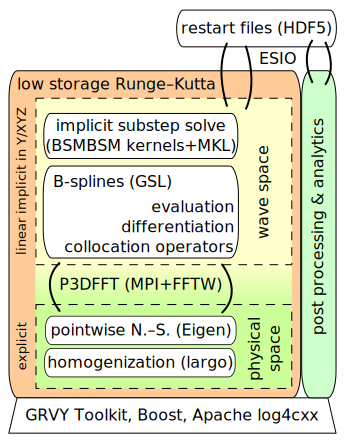
\includegraphics[width=0.6\textwidth]{SuzerainDesignOverview}
\\
\caption{%
    Architecture for the spectral
    simulation framework Suzerain\label{fig:suzeraindesign}
}
\end{figure}

\begin{figure}
\centering
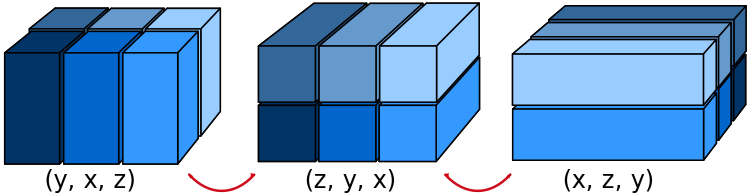
\includegraphics[width=.95\linewidth]{PencilTransposeSchematic}
\\
\caption[Parallel data movement stages for pencil decompositions]{%
  A pencil decomposition maps $O(N^2)$ data to $O(N^3)$ MPI ranks using two
  \texttt{MPI\_Alltoall}-like global communication phases depicted with red
  arrows.  Each color represents the data owned by a single rank in each
  configuration.  \label{fig:penciltranspose}
}
\end{figure}

The high-level design of Suzerain is depicted in \autoref{fig:suzeraindesign}.
Best-of-breed third party libraries were used when it was advantageous to
do so.  Computing one Runge--Kutta substep
per~\eqref{eq:generaloperatormasssubstep} transforms state from wave space to
physical space and transforms residuals back using P3DFFT~\citep{P3DFFTweb}.  These parallel
transposes, depicted in \autoref{fig:penciltranspose}, provide the natural
domain decomposition which arises from the Fourier/B-spline spatial
discretization~\eqref{eq:spatial_discretization}.  The communication and
computation characteristics of those operations are crucial for scalability.

B-spline operators were formed using the GNU Scientific Library
(GSL)~\citep{Eaton2008GNU}.\footnote{%
    The author is a committer for the GSL project.
}
The banded implicit solves in Algorithm~\ref{alg:step} required custom compute
kernels to assemble rescaled B-spline operators into large-bandwidth,
complex-valued BSMBSMs per \autoref{sec:solutionimplicitoperator}.
Factorization and back-substitution are provided by
the Intel\textsuperscript{\textregistered} Math Kernel Library (MKL).\footnote{%
    By default, implicit solves employ a robust, LAPACK-like driver.  The user
    may also choose the vanilla \texttt{GBTRF/GBTRS} pair for speed, the more
    expensive \texttt{GBSVX} driver to monitor operator conditioning, or a
    custom banded driver routine inspired by \citet{Langou2006Exploiting}'s
    \texttt{DGESIRSV} permitting mixed precision operation and/or exploiting
    approximate factorizations.  While this last option provided verifiably
    correct results, reusing the $(k_n,k_m)$-dependent operator (see
    \autoref{fig:discreteimplicitop}) factorization along with iterative
    refinement to avoid nearby $(k_n',k_m')$ factorizations was not found to be
    superior to invoking \texttt{GBTRF} for every $(k_n,k_m)$ on the problems
    considered in this document.
}
Custom banded matrix-vector product kernels were prepared because
compiler-unrolled loops are appreciably faster than general-purpose
MKL routines at small bandwidths~\citep{Lee2013Petascale}.\footnote{%
    Note the matrix-vector product bandwidths are significantly
    smaller than that factorization problem bandwidths as discussed in
    \autoref{sec:solutionimplicitoperator}.
}
In physical space, pointwise
Navier--Stokes-related computations used Eigen~\citep{eigenweb}
to simplify expressing complicated expansions
like~\eqref{eq:linearized_pressure_gradient} and to facilitate accessing
vectorized intrinsics for performance.  When applied, the slow growth forcing
discussed in
Sections~\ref{sec:background_homogenization} and~\ref{sec:imposing_fpg} is
accomplished using largo, a standalone Fortran 90/C99 library developed by Victor
Topalian which is distributed with Suzerain.

The GRVY Toolkit~\citep{GRVYweb} was used for continuous performance monitoring
while extensions atop Apache log4cxx~\citep{log4cxxweb} provided rich, MPI-aware
logging of both application lifecycle events as well as the temporal evolution
of statistical quantities of interest.\footnote{The author is a committer for both
the GRVY Toolkit and Apache log4cxx projects.}  Input and output of
HDF5-based~\citep{hdf5} data files was performed using the
ESIO library~\citep{ESIOweb}, written as part of the current work and also
openly available.\footnote{\url{http://github.com/RhysU/ESIO}}  Operational
considerations like automated batch job output management and reactive tear down
in the event of job time expiration or queue-system-related interruption were
implemented to permit long simulations to run virtually unattended.

Absent from \autoref{fig:suzeraindesign} are the pervasive
computational science toolkits PETSc~\citep{Balay1997Efficient} and
Trilinos~\citep{Heroux2005Overview}.  During Suzerain's early design they were
investigated but six years ago it was unclear how to fit the techniques
from \autoref{sec:techniques} into them.  Three years ago, having learned more,
it became apparent that doing so was possible.  However, at that time, the
basic features either toolkit would have provided had already been long ago
implemented within Suzerain making porting a considerable effort
without immediately obvious benefits.  No port occurred.

In hindsight, not adopting a common toolkit into Suzerain's design was
suboptimal.  Gaining access to off-the-shelf, adaptive temporal schemes
would have permitted taking full advantage of the increased stability provided
by the wavenumber-dependent, linearly implicit operator implementation in the
streamwise and spanwise directions without concerns as to whether or not doing
so adversely impacts accurately capturing turbulent dynamics (see
\autopageref{eq:bigtimesteps} and, below, \autoref{sec:channel_runs}).  It
certainly would have largely rendered the work behind
\autoref{sec:wallnormaleigval} unnecessary as classical CFL stability estimates
would yield conservative initial guesses from which an adaptive scheme could
ramp up the time step to a maximally efficient value given well-quantified
accuracy requirements.  If found prohibitively expensive for production calculations,
adaptive schemes could be applied during simulation ``spin-up'' followed by
nonadaptive time advance using spin-up-informed time step choices.  Reactive
stability restrictions arising from spatiotemporal forcing would have been
seamlessly handled rather than requiring the step size safety factors listed
in \autoref{sec:bldata}.  Finally, and most importantly, skeletally
incorporating a ubiquitous toolkit could increase the likelihood and speed of
future Suzerain adoption by PETSc- or Trilinos-savvy developers thus
facilitating collaboration and providing better research returns for the time
invested in the code.


%%%%%%%%%%%%%%%%%%%%%%%%%%%%%%%%%%%%%%%%%%%%%%%%%%%%%%%%%%%%%%%%%%%%%%%%%%%%%%
\section{Testing and Verification}

Automated testing and code verification are essential as Suzerain is used to
produce data for model calibration.  Unit tests ensure lower level
routines behave as expected while a collection of higher-level tests verify
their proper integration.  MPI-parallel system tests check first for correct operation
and second, wherever applicable, for agreement with serial computations.
Serial/parallel consistency tests include the full application lifecycle
involving loading restart state, advancing time, computing statistics, and
storing state back to disk.  Gold solutions, which are known-correct results
calculated by earlier code revisions, permit detecting when changes
like implementing optimizations or switching compiler versions
unintentionally influence results.
The full test suite
was run daily on a Buildbot continuous integration server~\citep{Buildbot}
against both the GNU and Intel\textsuperscript{\textregistered} compilers.  At present, automated line and function coverage
exceeds 80\%.

%\subsection{The Method of Manufactured Solutions}

To verify that Suzerain correctly implemented Equations~\eqref{eq:nondim_model}, the method of manufactured solutions (MMS)
was employed.  The MMS adds to the governing equations new source
terms such that the exact -- manufactured -- solution is known \textit{a
priori}~\citep{Roache1984Symbolic, Steinberg1985Symbolic, MASA}.  New
manufactured solutions were created to fully test all terms in compressible
Navier--Stokes formulations like the present one~\citep{Ulerich2012MMS}.  The
particular solution instantiation appropriate for the current
nondimensionalization is recorded in Appendix~\ref{sec:mms}.

\begin{figure}[t]
\centering
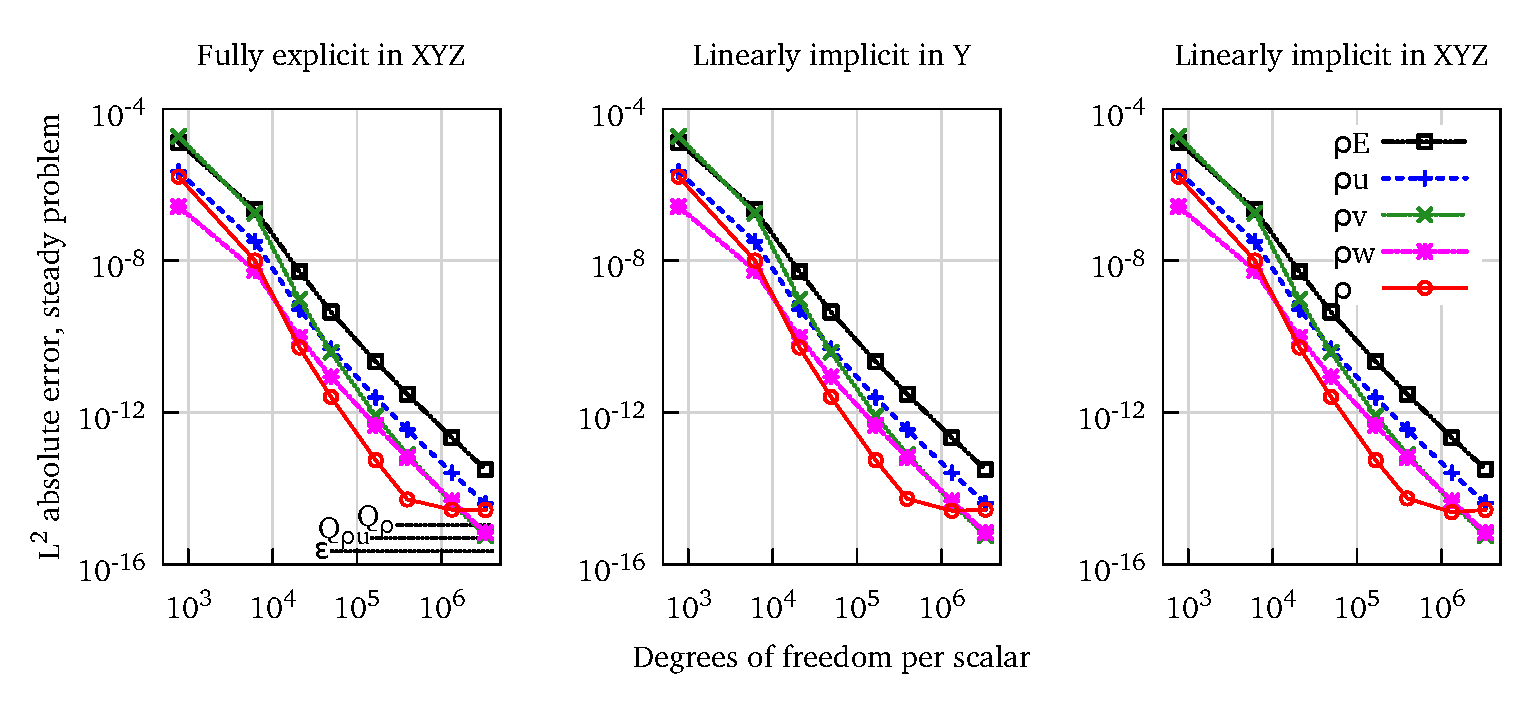
\includegraphics[width=\textwidth]{mms-convergence-steady}
\caption[Verification of Suzerain against a steady manufactured solution]{%
  Convergence behavior against a steady problem solved using each available
  Navier--Stokes operator implementation.  The wall-normal resolution ---
  piecewise-septic B-splines atop uniform breakpoints with 12, 24, 36, 48, 72,
  96, 144, and 192 collocation points --- governs the asymptotic order.  The
  three sample estimate~\eqref{eq:orderest} finds $k_0>7.34$ across $h=48$,
  $h/s=72$, and $h/t=96$ for all scalars.  Labels $Q_\rho$ and $Q_{\rho{}u}$
  indicate measured pointwise error in the floating point computations
  implementing manufactured forcing~\citep{Ulerich2012MMS}.  Beyond 96
  collocation points that forcing error reduces empirical convergence rates.
  For reference, label $\epsilon$ marks machine
  epsilon.\label{fig:convergence-steady}
}
%
\end{figure}

\begin{figure}[t]
\centering
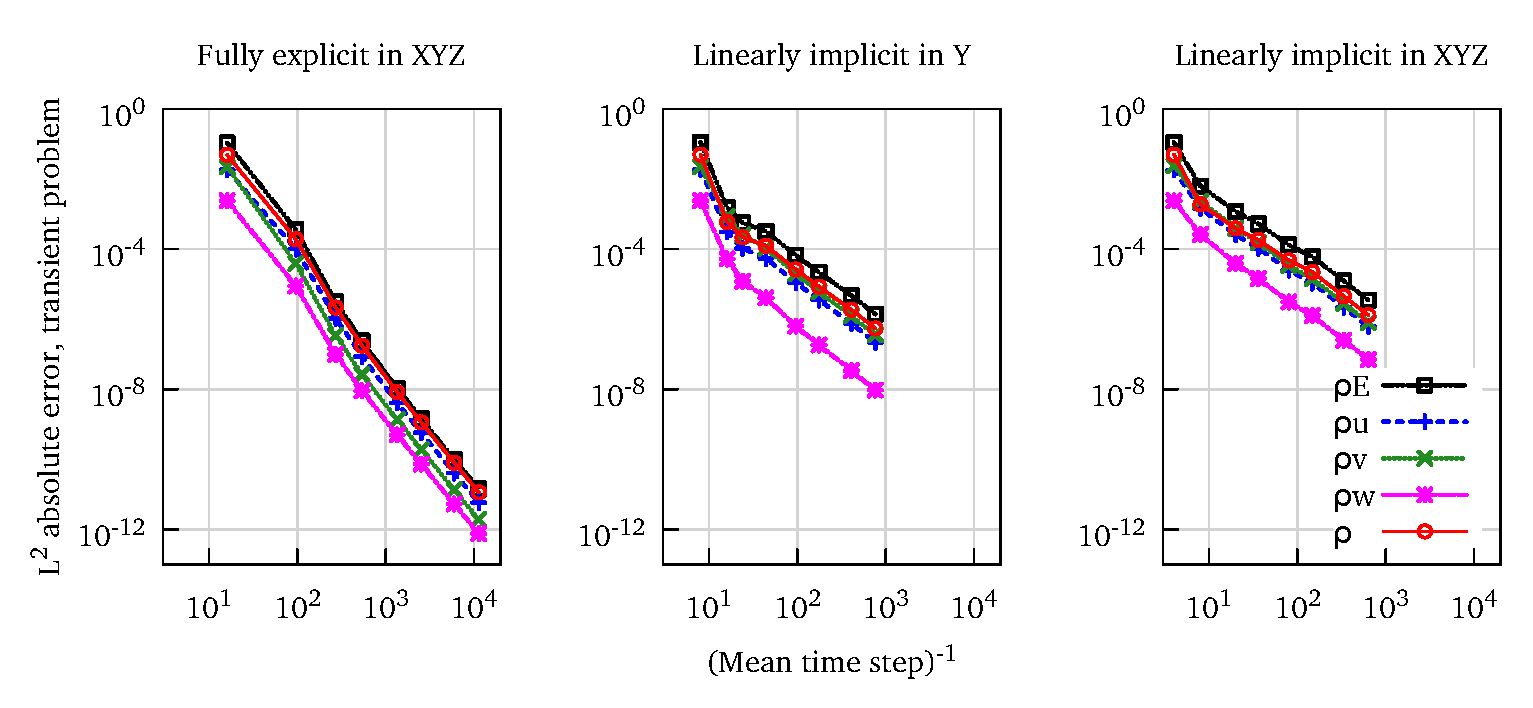
\includegraphics[width=\textwidth]{mms-convergence-transient}
\caption[Verification of Suzerain against a transient manufactured solution]{%
  Convergence behavior against a transient problem over 0.25 time units solved
  using each available Navier--Stokes operator implementation.  The same
  spatial resolutions from \autoref{fig:convergence-steady} were reused to
  force temporal refinement to be driven by stability concerns per
  \autoref{sec:stabilitycriteria}.  When fully explicit (left), stable time
  steps are small enough that pre-asymptotic, almost-spatial orders are
  recovered ($k_0>6.45$).  Wall-normal implicitness (center) exhibits $k_0>3.6$
  for $N_y\geq{}48$ while advancing linearly implicitly in three directions
  (right) shows $k_0>2.1$ for $N_y>72$.  Notice significant differences in
  step sizes occurring across the three
  implementations.\label{fig:convergence-transient}
}
\end{figure}

After the manufactured solution was constructed, three-sample observed order of
accuracy studies were conducted~\citep{Roy2005, Roache1998Verification}.
Assuming an approximation $A(h)$ shows an $h$-dependent truncation
error compared to an exact value $A$, \textit{viz.} $A - A(h) = a_0h^{k_0} +
a_1h^{k_1} + \cdots$, gives rise to the classical Richardson extrapolation
procedure.  Neglecting $O(h^{k_1})$ contributions, one can estimate the leading
error order $k_0$ by numerically solving
\begin{align}
  A &=
  \frac{t^{k_0}A\!\left(\frac{h}{t}\right) - A(h)}{t^{k_0}-1} + O(h^{k_1})
  = \frac{s^{k_0}A\!\left(\frac{h}{s}\right) - A(h)}{s^{k_0}-1} + O(h^{k_1})
  \label{eq:orderest}
\end{align}
given three approximations $A(h)$, $A(h/s)$, and $A(h/t)$ to $A$.  The $L^2$
norm of the absolute error in each scalar field was selected here.  On steady
problems, the wall-normal B-spline discretization error generally dominates that
arising from the spectral streamwise and spanwise Fourier basis truncation as
displayed in \autoref{fig:convergence-steady}.  On transient problems, the
linearly implicit temporal treatment can reduce the asymptotic convergence rate
to as low as second order as demonstrated in
\autoref{fig:convergence-transient}.

\begin{figure}
\centering
\includegraphics[width=\textwidth]{NRBC_rhome_y}
\caption[Verification of nonreflecting boundary conditions]{%
  The temporal evolution of mean pressure across the streamwise and spanwise
  directions as a function of wall-normal distance is depicted during a
  nonreflecting boundary condition test.  At $t=0$ the wall temperature is
  instantaneously dropped causing a pressure pulse to travel towards the upper
  boundary which it exits before $t=5$.  An acceptable reflection is seen
  traveling back towards the wall which it reaches around $t=8$.  The
  effectiveness of the approximately nonreflecting boundary can be contrasted
  with the subsequent pressure reflection from the isothermal wall which is
  faint but visible at $y=5/4$ when $t=10$. \label{fig:nrbc-verify}
}
\end{figure}

Two important code features were not verified via manufactured solutions.  Both
features are, of course, believed to be formulated and implemented correctly but
that belief is not based upon Figures~\ref{fig:convergence-steady}
or~\ref{fig:convergence-transient}.  The first feature was the nonreflecting
boundary treatment discussed in \autoref{sec:nrbc}.  The related
matrix-manipulating logic~\eqref{eq:dimeulertransformevolve_linearfact} was
exercised by automated tests.  A variety of two- and three-dimensional test
problems, like the one depicted in \autoref{fig:nrbc-verify}, were used to
assess proper boundary condition enforcement within the larger temporal
advancement scheme per \eqref{eq:dimeulertransformevolve_nonlinear} and
\eqref{eq:dimeulertransformevolve_linear}.
%
%Empirical reflection coefficients were not, however, assessed.
%
The second feature was the data exchange between the main solver in Suzerain and
the pointwise homogenized forcing computations coded in Topalian's
largo library.  The homogenization-agnostic data hand off between largo and
Suzerain was subjected to intensive code review followed by capturing results in
gold solution files to defend against regression.
%
%It was difficult to provide strong coverage of this code integration point
%without falling prey to excessive brittleness as the slow growth formulations
%evolved within the largo library.
%
Topalian provided automated, pointwise verification of the computations
inside largo.


%%%%%%%%%%%%%%%%%%%%%%%%%%%%%%%%%%%%%%%%%%%%%%%%%%%%%%%%%%%%%%%%%%%%%%%%%%%%%%
\section{Validation on Isothermal Channel Problems}
\label{sec:channel_runs}

To validate Suzerain, including its uncertainty and post-processing
capabilities, a collection of sub- through supersonic, low Reynolds number
isothermal channels was simulated~\citep{Ulerich2012Turbulence}.  The collection
followed computations by \citet{Coleman1995Numerical} which were further
investigated by \citet{Huang1995Compressible} to permit direct comparison with
their results.  A wide range of Mach numbers was simulated to permit investigating, later
in this chapter, the efficiency of the linear-implicit treatment documented in
\autoref{sec:implicitlytreatedterms}.
%
The data is openly archived as described in Appendix~\ref{sec:archiving}.

In channel flows a fluid is driven between two flat plates separated by a fixed
distance as shown in \autoref{fig:geometry}.  The
incompressible~\citep{Kim1987Turbulence, Hoyas2006Scaling, DelAlamo2003Spectra,
DelAlamo2004Scaling, Simens2009Highresolution, Hoyas2008Reynolds} and
compressible~\citep{Coleman1995Numerical, Huang1995Compressible, Li2001DNS,
Morinishi2005Study, Friedrich2007Compressible, Friedrich2004Turbulence,
Lechner2001Turbulent, Schwartz1987Perturbation} versions of this problem are
well-studied.  Half the plate separation distance is taken as reference length
$l_0$ so that nondimensionally $L_y=2$.  No slip, isothermal conditions are
enforced at the upper and lower boundaries.  Unlike the classical plane
Poiseuille flow in which a constant pressure gradient drives the fluid, in
Coleman-like channels the bulk streamwise momentum, $\int\rho{}u\,\mathrm{d}\!y,$
is constrained using a spatially uniform, time-varying body force $f$.  The
instantaneous bulk density is similarly fixed.  In contrast, the total energy is
not constrained so that the problem becomes energetically stationary only when
the mean work done by $f$ is balanced by the average heat transfer through the
walls.  To simplify comparison, the grid resolutions and domain size closely
follow \citet{Coleman1995Numerical} who found them to be adequate.  The domain
is small relative to more recent channels appearing in the
literature.

% Source data from http://turbulence.ices.utexas.edu/coleman/ with MD5:
%   40ded1a60f8d65a7282c5afaa8d43e10  coleman3k01.h5
%   65561dbb6918e828afed9cf31a61f600  coleman3k05.h5
%   73ee5929a5fc4b726e6095ffe1ed2589  coleman3k15.h5
%   f9147b944f908af9b4dfc86b000df89a  coleman3k30.h5
%   1581eee7c8e4ff4a227f67cdf8357235  coleman5k01.h5
%   12658b01075e5acd49098f519fb11918  coleman5k05.h5
%   25d4944b8729aa7308f65302279172fe  coleman5k15.h5
%   5113239ac101f2b7c357fc70f8f49721  coleman5k30.h5

% Number of flow throughs for KMM87 computed as follows:
%    t u_\tau / \delta \approx 10 (page 140 second to last paragraph)
%    \delta = 1
%    U_m / u_\tau = 15.63 (Table 1)
%    U_m = 1
%    L_x = 4*pi*\delta
% combining shows 12.43 flow throughs

\begin{table}
\makecommand{\z}{\phantom{0}}  % Facilitates column alignment
\makecommand{\Z}{\phantom{.0}} % Ditto
\centering
\caption[Isothermal channel simulations]{%
    Isothermal channel simulations performed with Suzerain
    v0.1.6.34-r45407.  For all cases, $\overline{\rho} = 1$,
    $\overline{\rho{} u} = 1$, $T_w = 1$, $\textrm{Pr} = \mu C_p
    / \kappa = 0.7$, $\alpha=0$ for $\mu_B=\alpha\mu$, $\mu /
    \mu_0={\left(T / T_0\right)}^\beta$, and $\gamma = C_p / C_v =
    1.4$.  Extents were $L_x=4\pi$, $L_y=2$, $L_z=4\pi/3$ employing
    $N_x=192$ and $N_z=168$ Fourier modes and a piecewise-septic
    B-spline basis with $N_y$ collocation points stretched per
    the hyperbolic tangent parameter ``$\tanh$'' following~\eqref{eq:htstretch2}.  By definition,
    $\textrm{Re} = \overline{\rho{}u}\left(L_y / 2\right) / \mu_w$,
    $\textrm{Ma} = \bar{u} / a_w$.  Simulations by
    \citet*{Kim1987Turbulence} and \citet*{Coleman1995Numerical} are
    shown for comparison.\label{tbl:table_channel}
}
{\renewcommand{\tabcolsep}{0.435em}
\begin{tabular}{cccccccccccr}
Case                                     & % Simulation input parameters
$\textrm{Re}$                            &
$\textrm{Ma}$                            &
$\beta$                                  &
$N_y$                                    &
$\tanh$                                  &
$\textrm{Re}_\tau$                       & % Details from post-processing
$\Delta{}x^{+}$                          &
$y_{1}^{+}$                              &
$y_{10}^{+}$                             &
$\Delta{}z^{+}$                          &
\shortstack[c]{Flow\\throughs}
\\
\toprule\toprule
%id       &  Re    &  Ma    &  beta  &  Ny     &  tanh  &  Re &  x+    &  y+1   & y+10  &  z+   &   Flowthroughs       \\
c03k01    &  3000  &  0.1   &  \nicefrac{2}{3} &  128  &  2.25  & 191 &  12.5  &  0.22  & 11.9  & \z5.0 &   15.6       \\
c03k05    &  3000  &  0.5   &  \nicefrac{2}{3} &  128  &  2.25  & 194 &  12.7  &  0.22  & 12.1  & \z5.1 &   15.7       \\
\rowcolor{yellow}
c03k15    &  3000  &  1.5   &  \nicefrac{2}{3} &  128  &  2.25  & 222 &  14.6  &  0.26  & 13.8  & \z5.8 &   11.9       \\
c03k30    &  3000  &  3.0   &  \nicefrac{2}{3} &  128  &  2.25  & 297 &  19.4  &  0.34  & 18.5  & \z7.8 &   15.5       \\
\midrule
c05k01    &  5000  &  0.1   &  \nicefrac{2}{3} &  144  &  2.50  & 298 &  19.5  &  0.26  & 14.2  & \z7.8 &   11.1       \\
c05k05    &  5000  &  0.5   &  \nicefrac{2}{3} &  144  &  2.50  & 303 &  19.8  &  0.26  & 14.4  & \z7.9 &   11.6       \\
c05k15    &  5000  &  1.5   &  \nicefrac{2}{3} &  144  &  2.50  & 349 &  22.8  &  0.31  & 16.6  & \z9.1 &   13.2       \\
c05k30    &  5000  &  3.0   &  \nicefrac{2}{3} &  144  &  2.50  & 480 &  31.4  &  0.42  & 22.8  & 12.6  &   12.9       \\
\midrule
KMM87     &  2800  &  0\Z   &  0\Z             &  129  &        & 180 &  12\Z  &  0.05  & \z5.4 & \z7\Z &   12.4       \\
\rowcolor{yellow}
CKM95a    &  3000  &  1.5   &  0.7             &  119  &        & 222 &  17\Z  &  0.1\z & \z8\Z & 10\Z  &  $\geq 11.9$ \\
CKM95b    &  4880  &  3.0   &  0.7             &  119  &        & 451 &  39\Z  &  0.2\z & 17\Z  & 24\Z  &  $\geq 11.9$
\end{tabular}}
%
\\\vspace*{1.75em}
%
\begin{tabular}{cccccccccc}
Case                            &
$\textrm{Ma}_c$                 &
$\textrm{Ma}_\tau$              &
$\textrm{Re}_c$                 &
$y^\ast_c$                      &
$-\textrm{B}_q$                 &
${\rho}_w$                      &
${\rho}_c$                      &
${T}_c$                         &
${\mu}_c$
\\
\toprule\toprule
%id     &  Mac     &  Matau   &  Rec   &  {y*c} &  -Bq     &  rhow    &  rhoc    &  Tc      &  muc     \\
c03k01  &  0.116   &  0.006   &  3481  &  190   &  0.0003  &  1.002   &  0.9999  &  1.002   &  1.001   \\
c03k05  &  0.570   &  0.031   &  3387  &  185   &  0.0062  &  1.040   &  0.9973  &  1.043   &  1.028   \\
\rowcolor{yellow}
c03k15  &  1.497   &  0.081   &  2772  &  151   &  0.0496  &  1.365   &  0.9780  &  1.391   &  1.246   \\
c03k30  &  2.240   &  0.119   &  1765  &  \z94  &  0.1486  &  2.494   &  0.9278  &  2.666   &  1.923   \\
\midrule
c05k01  &  0.115   &  0.006   &  5752  &  297   &  0.0002  &  1.002   &  0.9999  &  1.002   &  1.001   \\
c05k05  &  0.566   &  0.029   &  5606  &  288   &  0.0058  &  1.041   &  0.9979  &  1.042   &  1.028   \\
c05k15  &  1.477   &  0.077   &  4585  &  238   &  0.0464  &  1.366   &  0.9835  &  1.385   &  1.242   \\
c05k30  &  2.202   &  0.116   &  2974  &  157   &  0.1436  &  2.486   &  0.9500  &  2.598   &  1.890   \\
\midrule
KMM87   &  0\Z\z\z &  0\Z\z\z &  3300  &  180   &  0\Z\z\z &  1\Z\z\z &  1\Z\z\z &  1\Z\z\z &  1\Z\z\z \\
\rowcolor{yellow}
CKM95a  &  1.502   &  0.082   &  2760  &  151   &  0.049   &  1.355   &  0.980   &  1.378   &  1.252   \\
CKM95b  &  2.225   &  0.116   &  2872  &  150   &  0.137   &  2.388   &  0.952   &  2.490   &  1.894
\end{tabular}
\end{table}

%
The channels simulated, including resolution details and various quantities of
interest, are reported in \autoref{tbl:table_channel}.  In the table, wall and
centerline quantities have subscripts $w$ and $c$.  Superscript ${+}$ denotes
normalization by the viscous length scale $\delta_\nu = \mu_w / \rho_w / u_\tau$ or the friction
velocity $u_\tau = \sqrt{\tau_w / \rho_w}$ where the wall shear stress
$\tau_w = \left(\mu \partial_y u\right)_w$.  The friction Reynolds number
$\Reynolds[\tau]{}$ and friction Mach number $\Mach[\tau]{}$ are given by
$y_c/\delta_\nu$ and $u_\tau/a_w$.  Superscript $\ast$ marks
scaling by semi-local units
%
using either $u^\ast_\tau = \sqrt{\tau_w / \rho}$ or $\delta^\ast_\nu = \nu / u^\ast_\tau$~\citep{Huang1995Compressible,Morinishi2005Study}.
%which are similar to
%$\delta_\nu$ and $u_\tau$ except that local density and viscosity are used in
%lieu of wall values.
The nondimensional heat flux is denoted by
$B_q$~\citep{Bradshaw1977Compressible}.  The column ``flow throughs'' conveys
the time over which the data ensemble was collected, divided by the time required
for the bulk flow to traverse the streamwise extent of the domain.
Linearly implicit operators were used in all three directions.

A direct comparison between the present results and those by
\citet{Coleman1995Numerical} can be made from the $\Reynolds=3000$, $\Mach=1.5$
cases c03k15 and CKM95a, which are highlighted in \autoref{tbl:table_channel}.
Aside from differences in the numerics,\footnote{%
    \citeauthor{Coleman1995Numerical} used a Fourier-Legendre spatial
    discretization and a third-order, four-substep temporal scheme
    by \citet{Buell1990Direct}.
}
in the upper half of the table the only appreciable parameter differences
between these two cases are the wall normal resolution ($\Delta{}y^{+}_{10}$ of
$13.8$ vs $8$) and the viscosity power law exponent ($\beta$ of $2/3$ versus
$0.7$).  One-dimensional Fourier spectra at $y\approx{}0.04$ and $y\approx{}1$
(not shown) compare favorably indicating the former difference is benign.  The
latter difference was deliberate as it produces data mildly more appropriate for
high temperature environments as demonstrated by \autoref{fig:Svehla1962}.  In
the lower half of the table, discrepancies between these two particular
simulations range from $0.43\%$ ($\Reynolds[c]{}$) to $1.3\%$ ($\Mach[\tau]$).
Minor disagreement is expected per the noted parameter differences but
additional root causes are further explored below.  Though nominally possible,
another comparison between rows c05k30 and CKM95b is not valid as the c05k30
hyperbolic tangent stretching parameter was too small causing insufficient
near-wall resolution as assessed by spectra (not shown).

%\begin{figure}
%\centering
%\includegraphics[width=0.495\textwidth]{c03k15_figure7a}
%\hfill
%\includegraphics[width=0.495\textwidth]{ckm95_figure7a}
%\\
%\caption[Isothermal channel profile comparison at $\Reynolds=3000$, $Mach=1.5$]{%
%  Comparison of mean primitive quantity profiles from present simulation c03k15 (left)
%  and CKM95a (right), reproduced from \citet{Coleman1995Numerical}.
%  \label{fig:qual_r3km15_comp}
%}
%\end{figure}

\begin{figure}
\centering
\includegraphics[width=\textwidth]{profile-c03k15}
\caption[Profiles with quantified uncertainty for $\Reynolds=3000$, $\Mach=1.5$ channel]{%
    Reynolds-averaged primitive profiles (upper left) and Favre-averaged
    Reynolds stresses scaled by semi-local units~\citep{Huang1995Compressible}
    (lower left) with estimated standard errors as a fraction of mean (upper
    right, lower right) from simulation c03k15.\label{fig:basic3k15}
    % COMPARE ColemanJFM1995 Figure 7a
}
\end{figure}

Based on techniques from \autoref{eq:uqaccounting}, mean primitive quantity and
Favre-averaged Reynolds stress profiles along with pointwise uncertainty
estimates appear for simulation c03k15 in \autoref{fig:basic3k15}.  The
autoregressive technique by \citet{Oliver2014Estimating} was used to estimate
pointwise sampling error at each wall-normal collocation point based on 383
instantaneous averages over the two Fourier directions.  In the upper right of
the figure, uncertainties normalized by mean velocity $\bar{u}$, temperature
$\bar{T}$, and viscosity $\bar{\mu}$ are higher near the wall due to both
turbulent fluctuations and the fact that the mean values take minima there.  The
largest normalized uncertainties in mean density $\bar{\rho}$ are slightly
offset from the other peaks because the mean value increases as one approaches the wall.  Uncertainty
in $\bar{u}$ is appreciably larger than that for the thermodynamic quantities
consistent with their relative root-mean-squared magnitudes \citep[Figures~10
and~18]{Coleman1995Numerical}.
%
We were unable to locate a published uncertainty estimate by Coleman or his
collaborators for the CKM95a simulation data against which to compare.
%
Uncertainty in near-wall $\bar{u}$ and centerline $\bar{u}$ are roughly 6 and
1.5 times larger, respectively, than analogous incompressible results from
\citet{Oliver2014Estimating} when both are scaled by the inverse root of the
number of flow throughs in the ensemble.  This difference will be addressed in
more detail below.

In the lower right of the figure, sampling errors have been propagated into the
derived, Favre-averaged quantities via the Taylor series
method~\eqref{eq:tsm_var1}.  Uncertainty in the density-weighted Reynolds
stresses is approximately an order of magnitude higher than was found for
quantities like $\bar{u}$.  The stresses are partially less certain because
their calculation takes as input higher order moments which are inherently less
well-known given a finite sampling window.  A second factor contributing to
uncertainty in the stresses is that the definition of
$\widetilde{u_i^{\prime\prime}u_j^{\prime\prime}}$ involves scaling by
$\bar{\rho}^{-1}$ which magnifies uncertainty when applying the Taylor
expansion~\eqref{eq:tsm_var1}.

A third factor contributing to relatively higher uncertainties in the Reynolds
stress was an operational error.  It was discovered because the \emph{a
posteriori} uncertainty estimates showed larger-than-anticipated asymmetries
about the channel centerline though mean values did not.
%
Given the solver verification results in \autoref{fig:convergence-steady} and
\autoref{fig:convergence-transient}, an error in the implementation of the
post-processing logic initially was suspected but no symmetry-breaking issues
were uncovered there.
%
On careful review, all new simulations in \autoref{tbl:table_channel} showed
evidence of infrequent, mild near-wall temporal instability though they used
the empirical B-spline operator stability estimates
with the safety factor
of 0.72.
%
The problem was diagnosed from temporal traces of the instantaneous global
minimum of the streamwise momentum--- a simulation monitoring feature not yet
implemented when the empirical stability estimates were created.  Channel flows
exhibit small, pointwise-negative velocities near the wall and it is exactly
these locations where linear-implicitness about the instantaneous mean state,
as described in \autoref{sec:implicitlytreatedterms}, is most subject to
stability problems when time steps are too large.
%
Implicit treatment in only the wall-normal direction also showed, under review,
the same symptom indicating that the operator stability estimates from
\autoref{sec:wallnormaleigval} were too aggressive for the safety factor
0.72.\todo{Sane threshold was 0.40 for c03k15}

Marginal temporal instability was manifest in asymmetric uncertainty estimates
because independent, short-duration instability events occurred infrequently
enough near each wall that over O(10) flow throughs in a small domain their
impact was not distributed evenly between the upper and lower halves of the
channel.
%
As a consequence of this mistake, figures in the present section do not merge
the upper and lower portions of the channel as is commonly done.  Not merging
data across the centerline accounts for a factor of 1.5 increase in $\bar{u}$
uncertainty relative to aforementioned scaled results by
\citet{Oliver2014Estimating}.
%
The remaining threefold increase in near-wall $\bar{u}$ uncertainty relative to
their work is at least partially due to these infrequent events.  That said,
it is also partially attributed to the growth in root-mean-squared $u$
fluctuations as the Mach number increases.
%
The same time step size mistake certainly contributes to the disagreement
between cases c03k15 and CKM95a found in \autoref{tbl:table_channel} and the
jaggedness of the near-wall uncertainty curves in the upper right of
\autoref{fig:basic3k15}.

\begin{figure}[tb]
\centering
\includegraphics[width=0.85\textwidth]{tke3k15}
\caption[Turbulent kinetic energy budgets for $\Reynolds=3000$, $\Mach=1.5$ channel]{%
    Budgets for the turbulent kinetic energy~\eqref{eq:fans_tke}
    for channel simulation c03k15 normalized as by~\citet[figure
    16a]{Huang1995Compressible}.  Omitted terms relative
    to~\eqref{eq:fans_tke} are a factor of 25 times smaller than maximum
    production.~\cite{Guarini2000Direct}\label{fig:tke3k15}.
    % COMPARE HuangJFM1995 Figure 16
}
\end{figure}

Term-by-term budgets for the turbulent kinetic energy~\eqref{eq:fans_tke}
in \autoref{fig:tke3k15} support the conclusion that time
discretization errors are appreciable in simulation c03k15.  Qualitatively, all
terms show expected trends.  However, relative to \citet[Figure
16a]{Huang1995Compressible}, approximately 5\% too much turbulent dissipation,
$\bar{\rho}\epsilon/\Reynolds$, is present at the wall along with a
counterbalancing increase in turbulent work.  \citet{Coleman2010Primer} linked
increased dissipation with temporal inaccuracy when Runge--Kutta schemes are
used.  Other terms are similarly affected.  For example, peak production $-\bar{\rho}
\widetilde{u^{\prime\prime}\otimes{}u^{\prime\prime}} : \nabla\tilde{u}$ is
roughly 10\% lower than \citeauthor{Huang1995Compressible} reported.
However, Suzerain's post-processing logic and the overall budget balance
are sound because the pointwise turbulent kinetic energy equation residual,
is appropriately small.


%%%%%%%%%%%%%%%%%%%%%%%%%%%%%%%%%%%%%%%%%%%%%%%%%%%%%%%%%%%%%%%%%%%%%%%%%%%%%%
\section{Performance and Scalability}
\label{sec:performance}

This section first discusses the efficiency of three available Navier--Stokes
operator implementations, briefly compares Suzerain's performance against a
highly tuned incompressible channel code, and lastly examines Suzerain's
scalability on production homogenized boundary layer simulations.  All
performance measurements were made on the Lonestar4 supercomputer at the Texas
Advanced Computing Center (TACC) as it will be the resource used for
production simulations in subsequent chapters.  Each compute node on Lonestar
contains 2~hex-core Intel\textsuperscript{\textregistered} Xeon\textsuperscript{\textregistered}~5680 3.33~GHz
processors and 24~GB of DDR3-1333~MHz memory.  Every core was used as a separate
MPI rank as Suzerain presently is not OpenMP-enabled.  Compute nodes are
interconnected in a fat-tree topology using Mellanox\textsuperscript{\textregistered}
InfiniBand\textsuperscript{\texttrademark} switches running at quad data rates of 40~Gbits/second.
Compilation was performed with version 11.1 20101201 of the
Intel\textsuperscript{\textregistered} compilers at optimization level~3 with host-specific
extensions enabled.

The efficiency of the fully explicit, linearly implicit in the wall-normal
direction, and linearly implicit in three directions operators were benchmarked
and are reported in \autoref{tbl:channel_performance}.  Efficiency was
measured as the amount of wall time required to advance one nondimensional time
unit because that physics-oriented metric directly translates into the expense
of acquiring converged turbulence statistics.  Another metric, wall time per
time step, will be presented later alongside scalability results.  Centerline
Mach numbers across the eight cases considered vary by nearly a factor of
twenty.   This broad range permits assessing efficiency for widely varying
acoustic-versus-convective restrictions as well as significant differences in
thermodynamic property fluctuation magnitudes.

\begin{table}
\centering
\makecommand{\z}{\phantom{0}}  % Facilitates column alignment
\caption[Relative efficiency of the Navier--Stokes operator implementations]{%
    Normalized wall time to advance simulation one nondimensional time unit
    using each of the available Navier--Stokes operator implementations.  Cases,
    defined in \autoref{tbl:table_channel}, were executed with Suzerain
    v0.1.6.34-r45407 using 12 nodes of Lonestar4.\label{tbl:channel_performance}
}
\begin{tabular}{cccc}
Case &
\shortstack[c]{Linearly implicit\\XYZ} &
\shortstack[c]{Linearly implicit\\Wall-normal} &
\shortstack[c]{Fully explicit}
\\
\toprule\toprule
%id     &  rhome_xyz  &  rhome_y  &  explicit
c03k01  &  \z1.0      &  11.0     &  49.5   \\
c03k05  &  \z1.0      &  \z2.9    &  10.3   \\
c03k15  &  \z1.0      &  \z1.3    &  \z3.7  \\
c03k30  &  \z1.0      &  \z1.4    &  \z2.0  \\
\midrule
c05k01  &  \z1.0      &  \z8.7    &  48.7   \\
c05k05  &  \z1.0      &  \z2.5    &  10.4   \\
c05k15  &  \z1.0      &  \z1.7    &  \z4.4  \\
c05k30  &  \z1.0      &  \z1.3    &  \z2.3  \\
\end{tabular}
\end{table}

On the eight cases examined, linear implicitness in three directions produced
time to solution speedups of 1.3--11x relative to treating only the wall-normal
direction implicitly.  The speedup improved as the Mach number decreased because
the more implicit operator mitigates streamwise and spanwise acoustic stability
concerns that would otherwise dominate at those conditions.  The measurable
speedup in higher speed channels is perhaps counterintuitive as the more
implicit
implementation requires matrix assembly and factorization for every $(k_m, k_n)$
wavenumber pair while the second fastest does not.  Though factorization has a
much higher asymptotic complexity than assembly, at this resolution the former
takes only twice the wall time of the latter.  Factorization of the assembled
matrices, here possessing bandwidth 69, has a favorable memory access pattern in
contrast with the assembly kernels and consequently performs comparatively well
despite the larger number of floating point operations it requires.
%
%%One additional benefit of increased implicitness is that it reduces
%%the number of \texttt{MPI\_Alltoall}-like parallel communication phases
%%required per simulation time unit during which no useful computations
%%are performed.

The above conclusions are what prompted selecting implicitness in three
directions for the isothermal channel simulations discussed in the prior
section.  Note that though less aggressive time step safety factors than 0.72
were in that section concluded to be required, safety factor reductions impact both
available implicit treatments fairly equitably and therefore do not grossly
upset their relative efficiencies.  Some simulations performed as part of the
next two chapters will use only wall-normal implicitness because they were not
limited by streamwise or spanwise stability thus making wavenumber-dependent
linear algebra detrimental to time-to-solution efficiency.  In summary, having both
types of implicitness available in Suzerain as equally viable options permits
the code to effectively address the wide range of flow conditions studied.

To assess the performance of Suzerain as a direct numerical simulation
framework, we compared it against the highly optimized channel
code PoongBack~\citep{Lee2013Petascale, Lee2014Experiences}, written by
Myoungkyu Lee.  PoongBack is a comparatively monolithic Fortran code for solving
the incompressible Navier--Stokes equations.  Like
Suzerain, PoongBack uses a Fourier--Galerkin/B-spline collocation spatial
representation in conjunction with a three-stage, low-storage semi-implicit
advance.  The \citet{Kim1987Turbulence} Navier--Stokes formulation advances two scalar state
variables in time requiring three wave-to-physical parallel Fourier transforms
and five physical-to-wave transforms per time step.  Every $(k_m, k_n)$
wavenumber pair requires multiple linear solves but the operators do not couple
multiple equations and require relatively uncomplicated matrix assembly to form.
Unlike Suzerain, PoongBack uses wholly custom linear algebra routines,
wholly custom, quadrature-aware parallel Fourier transforms built atop FFTW
3.3's MPI capabilities, and hybrid MPI/OpenMP parallelism.  The comparison is
apt because many of Lee's improvements could be adopted by Suzerain if
performance improvements are required for future work.

Mimicking the resolution from our simulation c03k01, Lee
performed an $\Reynolds[\tau]=180$ simulation on 12 nodes of Lonestar4 using 6
OpenMP threads per processor.  PoongBack took 0.1299 seconds to complete one
Runge--Kutta step.  The timing of high-level tasks from our c03k01 case were
collected and then scaled by the frequency with which they are required to
advance the \citet{Kim1987Turbulence} formulation.  For example,
the wall time P3DFFT required to transform 30+ scalar fields from wave space to
physical space was scaled to reflect PoongBack only needing to perform that task
for three fields.
%
Physical space nonlinear product costs were scaled by the ratio of the number of
scalar equations involved, a conservative choice because the incompressible
system of equations is considerably less complex than the
compressible one.
%
% Comparing notes with MK on 2 July 2014
%
% Code      Operation Number/Substep Complexity
% Suzerain  Factorize 1              S**3
%           Backsub   1              S**2
%           Matvec    33             1
%           Assembly  1              S**2
%           Wave2Phys 33             1
%           Phys2Wave 4 (channel)    1
%           Nonlinear 1              5
% PoongBack Factorize 6              S**1
%           Backsub   29             1
%           Matvec    41             1
%           Assembly  2              1
%           Wave2Phys 3              1
%           Phys2Wave 5              1
%           Nonlinear 1              2
%
Scaling for linear algebra tasks, including matrix-vector products, matrix
assembly, back substitution, and factorization, reflected both the relative
number of tasks performed during one substep as well as relative code-to-code
operation costs arising from differences in equation coupling.  For example,
factorization costs were scaled by $6/5^3$ as, per wavenumber pair, PoongBack
performs six single-equation factorizations while Suzerain performs one
monolithic factorization with a leading-order, \texttt{S}-dependent cubic
complexity~\eqref{eq:bsmbsm_factorization}.

After rescaling, each hypothetical
Suzerain time step solving the incompressible \citeauthor{Kim1987Turbulence}
formulation required 0.629 seconds representing a 4.8x slowdown relative to
PoongBack.  About 30\% of the hypothetical wall time per time step would be
spent on parallel transposes with the vast majority of the remainder consumed by
banded algebraic operations.  Less conservative estimates of the nonlinear
product costs incurred in physical space bring the hypothetical slowdown as low
as $4\times$.  The hypothetical slowdown is larger than hoped but reasonable---
Lee took in excess of a year to produce PoongBack with much of that time spent
crafting and tuning formulation-specific banded algebraic logic to which he
attributes an overall speedup of $2\times$ (personal communication).

% State:  512x256x256 by 5 fields by 8 bytes per double
% Padded: 768x256x384 by 33(down)+5(up) fields across 3 substeps by 8 bytes
%
Suzerain's strong scalability as well as timings for the three available
Navier--Stokes operator implementations are shown in \autoref{fig:scaling}.
The problem size studied, which could run on as few as 24 MPI ranks,
corresponds to the production grid to appear in \autoref{sec:bldata}.  The state
is only 168 million real-valued degrees of freedom (1.3~GB) but each
full Runge--Kutta step required P3DFFT to transmit and fast Fourier
transform 69~GB of information.  Scalability from 24 to 48 ranks was not
good but from 48 to 384 ranks operator-specific parallel efficiencies
exceeded 93.3\%.  Within this sweet spot, advancing linear implicitly in
one or three directions took 107--110\% or 152--155\% of the wall time
of a fully explicit time step, respectively.

\begin{figure}[tb]
\centering
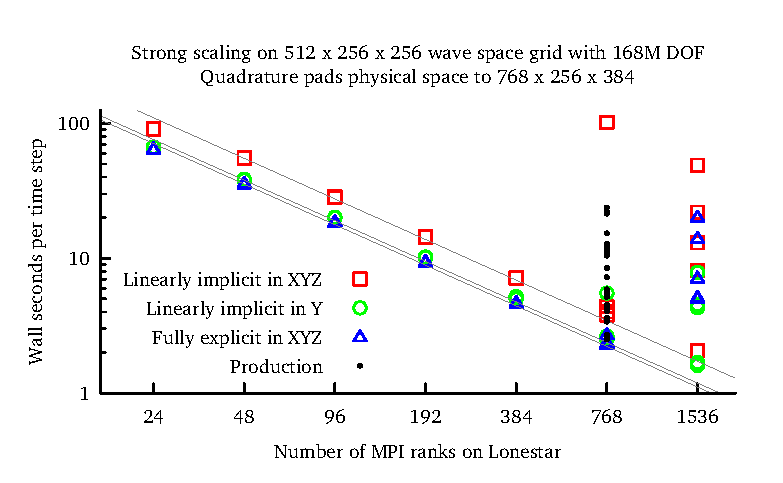
\includegraphics[width=0.85\textwidth]{scaling}
\caption[Strong scalability of Suzerain on TACC's Lonestar4 resource]{%
    Strong scalability on a homogenized boundary layer scenario.  At least three
    samples are present for each rank count and Navier--Stokes operator
    implementation.  Workload is well-balanced at all rank counts.
    Grey lines indicate perfect parallel efficiency based upon 48-rank
    performance.  Production timings, here implicit in only the
    wall-normal direction, included the overhead of writing statistics and
    checkpoint files.\label{fig:scaling}
}
\end{figure}


At 768 and 1536 ranks, job-to-job measurements of the wall seconds per time step
became highly variable.  We attribute the behavior either to such batch jobs
often executing on compute nodes separated widely on Lonestar4's fat-tree
interconnect or to some other intermittent network issue.  Though some
variability was always present at these rank counts, atop an unchanged Suzerain
binary it became dramatically worse after a Lonestar4 system maintenance on 27
May 2014.  The better jobs measured after that date exhibited coefficients of
variation between 2--4\% for the time it took P3DFFT to transform a single
scalar field while the worse jobs exceeded 500\%.  P3DFFT scalability problems
on Lonestar4 at 768 and 1536 ranks was also observed by \citet{Lee2013Petascale}
though they encountered nothing so severe.  Despite these issues and due to
time-to-solution considerations, production simulations were executed on 768
ranks because, when provided with a favorable network fragment, job efficiency
moving from 384 to 768 ranks could approach 100\%.  \autoref{fig:scaling}
includes laggard production jobs that, when detected, were manually stopped to
conserve compute resources.

%%As mentioned, the problem decomposition provided by the parallel transpose
%%library dictates scalability.  Balancing communication and computation tradeoffs
%%in conjunction with resolution requirements can be difficult and lead to
%%suboptimal scaling as above.  One promising approach, now deployed in a
%%hero-class, incompressible DNS code by \citet{Lee2013Petascale}, is adding
%%on-rank parallelism using OpenMP as well as FFTW's OpenMP-aware, autotuned
%%parallel transposes.  Hybrid parallelism allows greater flexibility in mapping
%%workloads to increasingly common many-core compute nodes.  An alternative
%%transpose library to P3DFFT, called ``underling'' and written as part of this
%%work, will allow seamlessly taking advantage of FFTW MPI's autotuned
%%capabilities~\citep{Frigo2005Design}.

%%Lastly, preliminary numerical analysis suggests that taking linearization
%%references about maximum rather than mean kinematic viscosities may
%%provide additional diffusive stability.  This analysis is to be hardened
%%and implemented as well.
